\chapter{Manuscript 2}


\vspace{3\parsep} %% Add triple space at start of chapter
% the above code is only needed if the start of the chapter goes from title to text without the initial starting of a \section{.}

\lipsum[1]

\section{Background}
\lipsum[1]

\section{Method}

\subsection{Participants}
\lipsum[1]

\subsubsection{Sample size determination} 
\lipsum[1]

\subsection{Measures}
\lipsum[1]

\subsection{Research Design}
\lipsum[1]




\section{Results}



\ref{tab:LongTable} gives an example of using a long table.





\newpage
\begin{longtable}{@{\extracolsep{\fill}}lcc}
\caption[A Long Table Example]{A Long Table Example} \label{tab:LongTable} \\

\toprule \multicolumn{1}{l}{Variables} & \multicolumn{1}{c}{Model} & \multicolumn{1}{c}{$\chi^2$} \\ \midrule
\endfirsthead


\toprule \multicolumn{1}{l}{Variables} & \multicolumn{1}{c}{Model} & \multicolumn{1}{c}{$\chi^2$} \\ \midrule
\endhead

\multicolumn{3}{r}{{(continued)}} \\  %The number in the multicolumn function needs to math the number of columns in the table for this to look OK
\endfoot

\bottomrule
\endlastfoot
A	&	1	&	21.85	\\
B	&	2	&	9.15	\\
C	&	3	&	20.58	\\
D	&	4	&	0.22	\\
E	&	5	&	0.60	\\
F	&	6	&	4.56	\\
G	&	7	&	1.08	\\
H	&	8	&	0.37	\\
I	&	9	&	7.77	\\
J	&	10	&	8.96	\\
K	&	11	&	5.21	\\
L	&	12	&	3.85	\\
M	&	13	&	3.34	\\
N	&	14	&	6.22	\\
O	&	15	&	8.11	\\
P	&	16	&	4.24	\\
Q	&	17	&	0.11	\\
R	&	18	&	3.86	\\
S	&	19	&	7.32	\\
T	&	20	&	2.75	\\
U	&	21	&	6.97	\\
V	&	22	&	5.98	\\
W	&	23	&	10.89	\\
X	&	24	&	5.61	\\
Y	&	25	&	3.51	\\
Z	&	26	&	7.17	\\
\end{longtable}

NOTE: There is another long table in Appendix \ref{app:con} as an extended example.

\subsection{Participants}
\lipsum[1]


Here is another example of a figure included in text.
Figure \ref{fig:srmrb} shows you how to include a note under a figure and still get the caption to be the correct length onthe figure list page. 
This is done by putting the caption you want to appear on the list page in square brackets [.] then putting the full caption with the note in the curly brackets.
This stupid process is needed so that the note aligns with the caption correctly. 

\begin{figure}[!tbp]
\centering
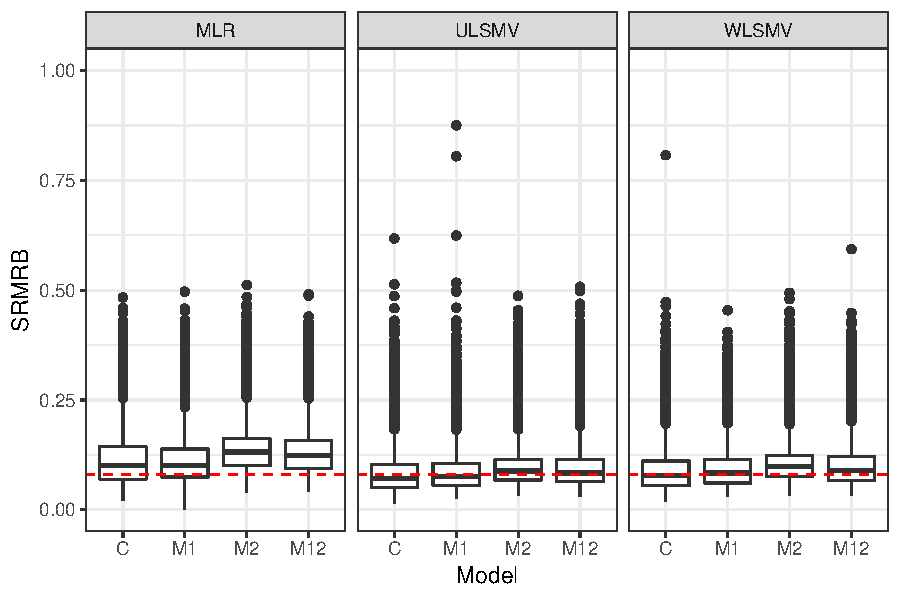
\includegraphics[width=0.85\textwidth]{figure/srmrb_marginal_model_estimator}
\caption[Distribution of SRMRB across estimated models and estimators]{Distribution of SRMRB across estimated models and estimators.\\ \textit{Note.} Dashed (red) line represents the Hu \& Benter (1999) commonly reported cut-off for SRMR at .08. We fixed the range to be 0,1 for viewing purposes; however, the max value we observed was 8.49.} \label{fig:srmrb}
\end{figure}

\subsection{Statistics and Data Analysis}
\lipsum[1]
\subsubsection{Missing Data}
\lipsum[1]

\subsubsection{Statistical Software}
\lipsum[1]

\section{Discussion}
\lipsum[1]


